\section{Direct synthesis}
\subsection{}

\begin{frame}
\frametitleTC{Introductory example}
\framesubtitleTC{as usual...}
\myPause
 \begin{itemize}[<+-| alert@+>]
 \item Consider the control loop we know, with $H(z)=1$ for simplicity:
       \begin{center}
        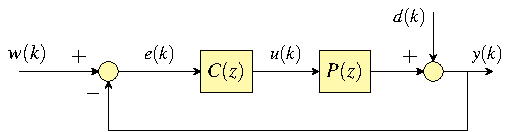
\includegraphics[width=0.50\columnwidth]{./Unit-04/img/ControlLoop-H1.pdf}
       \end{center}
 \item Take as process and controller, respectively,
       \begin{displaymath}
        P(z) = \frac{\mu}{z-p}, \qquad
        C(z) = \frac{1-\alpha}{\mu} \, \frac{z-p}{z-1},
       \end{displaymath}
 \item and analyse the obtained system.
 \end{itemize}
\end{frame}

\begin{frame}
\frametitleTC{Introductory example}
\framesubtitleTC{}
\myPause
 \begin{itemize}[<+-| alert@+>]
 \item We have a \TC{zero/pole cancellation} between controller and process, as the loop transfer function is
       \begin{displaymath}
        L(z) = P(z)C(z)
             = \frac{\cbcancel[gray]{\mu}}{\ccancel[red]{z-p}} \,
               \frac{1-\alpha}{\cbcancel[gray]{\mu}} \, \frac{\ccancel[red]{z-p}}{z-1}
             = \frac{1-\alpha}{z-1}
       \end{displaymath}
 \item Hence
       \begin{displaymath}
        G_{yw}(z) = \frac{L(z)}{1+L(z)}
                  = \frac{\frac{1-\alpha}{z-1}}{1+\frac{1-\alpha}{z-1}}
                  = \frac{1-\alpha}{\ccancel[green!80!black]{z-1}} \,
                    \frac{\ccancel[green!80!black]{z-1}}{z-1+1-\alpha}
                  = \frac{1-\alpha}{z-\alpha}.
       \end{displaymath}
 \item NOTE: the \textcolor{green!80!black}{simplification} in computing $G_{yw}$ is NOT a cancellation.
 \item[] \vspace{-0.75mm}To have a cancellation you need a system (block) with a zero say\\
       in $\overline{z}$, and \TC{\underline{ANOTHER}} system (block) with a pole in the same  $\overline{z}$\\
 \item[] \vspace{-0.75mm} --- as is the case with the \textcolor{red}{cancellation} in $L$ above.
 \end{itemize}
\end{frame}

\begin{frame}
\frametitleTC{Introductory example}
\framesubtitleTC{}
\myPause
 \begin{itemize}[<+-| alert@+>]
 \item Furthermore, as $H(z)=1$,
       \begin{displaymath}
        G_{yd}(z) = \frac{1}{1+L(z)}
                  = \frac{1}{1+\frac{1-\alpha}{z-1}}
                  = \frac{z-1}{z-1+1-\alpha}
                  = \frac{z-1}{z-\alpha}.
       \end{displaymath}
 \item You may -- should \smiley$\,$ -- remember that cancellations entail hidden parts for the affected system.
 \item Let us evidence and discuss the implications of this in the present\\
       case, by going through a state space analysis.
 \end{itemize}
\end{frame}

\begin{frame}
\frametitleTC{Introductory example}
\framesubtitleTC{State space formulation of the closed-loop system}
\myPause
 \begin{itemize}[<+-| alert@+>]
 \item First we express the process in state space form:
       \begin{displaymath}
        \left\{\begin{array}{rcl}
         x_P(k) &=& p x_P(k-1) + \mu u(k-1) \\
         y(k)   &=& x_P(k) + d(k)
        \end{array}\right.
       \end{displaymath}
 \item Then we rewrite the controller transfer function as a constant plus a term with numerator degree
       strictly less than denominator degree (check out the wxMaxima \texttt{divide} function):
       \begin{displaymath}
        C(z) = \frac{1-\alpha}{\mu} \, \frac{z-p}{z-1} 
             = \frac{1-\alpha}{\mu} \left( 1 + \textcolor{red}{\frac{1-p}{z-1}} \right)
       \end{displaymath}
 \item Then we treat the \textcolor{red}{strictly proper} term like $P(z)$ above, obtaining
       \begin{displaymath}
        \left\{\begin{array}{rcl}
         x_C(k) &=& x_C(k-1) + (1-p) e(k-1) \\
         u(k)   &=& \frac{1-\alpha}{\mu} x_C(k) + \frac{1-\alpha}{\mu} e(k)
        \end{array}\right.
       \end{displaymath}
 \end{itemize}
\end{frame}

\begin{frame}
\frametitleTC{Introductory example}
\framesubtitleTC{State space formulation of the closed-loop system}
\myPause
 \begin{itemize}[<+-| alert@+>]
 \item Joining the equations for $P$ and $C$ and those for the node that produces $e$, gives\\
       for the overall closed-loop system the scalar (not yet reduced to minimal) description
       \begin{displaymath}
        \left\{\begin{array}{rcl}
         x_P(k) &=& p x_P(k-1) + \mu u(k-1) \\
         x_C(k) &=& x_C(k-1) + (1-p) e(k-1) \\
         y(k)   &=& x_P(k) + d(k) \\
         u(k)   &=& \frac{1-\alpha}{\mu} x_C(k) + \frac{1-\alpha}{\mu} e(k) \\
         e(k)   &=& w(k) - y(k)
        \end{array}\right.
       \end{displaymath}
 \end{itemize}
\end{frame}

\begin{frame}
\frametitleTC{Introductory example}
\framesubtitleTC{State space formulation of the closed-loop system}
\myPause
 \begin{itemize}[<+-| alert@+>]
 \item For the process state we have
       \begin{displaymath}
        \begin{array}{rcl}
         x_P(k) &=& p x_P(k-1) + \mu u(k-1) \\
                &=& p x_P(k-1) + \mu \left( \frac{1-\alpha}{\mu} x_C(k-1) + \frac{1-\alpha}{\mu} e(k-1) \right) \\
                &=& p x_P(k-1) + (1-\alpha)x_C(k-1) + (1-\alpha) \left( w(k-1)-y(k-1) \right) \\
                &=& p x_P(k-1) + (1-\alpha)x_C(k-1) + (1-\alpha) w(k-1)\\
                & & - (1-\alpha) \left( x_P(k-1)+d(k-1) \right) \\
                &=& \left( p+\alpha-1 \right) x_P(k-1)
                    +(1-\alpha) x_C(k-1)\\
                & & +(1-\alpha) w(k-1)
                    -(1-\alpha) d(k-1)                 
        \end{array}
       \end{displaymath}
 \item while the controller state evolves according to
       \begin{displaymath}
        \begin{array}{rcl}
         x_C(k) &=& x_C(k-1) + (1-p) e(k-1) \\
                &=& x_C(k-1)\\
                & & + (1-p) \left( w(k-1)-x_P(k-1)-d(k-1) \right)\\
                &=& (p-1) x_P(k-1) + x_C(k-1)\\
                & & +(1-p) w(k-1)
                    -(1-p) d(k-1)  
        \end{array}
       \end{displaymath}
 \end{itemize}
\end{frame}

\begin{frame}
\frametitleTC{Introductory example}
\framesubtitleTC{State space formulation of the closed-loop system}
\myPause
 \begin{itemize}[<+-| alert@+>]
 \item Putting it all together, the closed-loop system in state space form reads
       \begin{displaymath}
        \left\{\begin{array}{rcl}
         \begin{bmatrix} x_P(k) \\ x_C(k) \end{bmatrix}
         &=& 
         \begin{bmatrix} p+\alpha-1 & 1-\alpha \\ p-1 & 1  \end{bmatrix}
         \begin{bmatrix} x_P(k-1) \\ x_C(k-1) \end{bmatrix}
         +
         \begin{bmatrix} 1-\alpha & \alpha-1 \\ 1-p & p-1  \end{bmatrix}
         \begin{bmatrix} w(k-1) \\ d(k-1) \end{bmatrix} \\
         \begin{bmatrix} y(k) \\ u(k) \end{bmatrix}
         &=& 
         \begin{bmatrix} 1 & 0 \\ \frac{\alpha-1}{\mu} & \frac{1-\alpha}{\mu} \end{bmatrix}
         \begin{bmatrix} x_P(k) \\ x_C(k) \end{bmatrix}
         +
         \begin{bmatrix} 0 & 1 \\ \frac{1-\alpha}{\mu} & \frac{\alpha-1}{\mu} \end{bmatrix}
         \begin{bmatrix} w(k) \\ d(k) \end{bmatrix} \\
        \end{array}\right.
       \end{displaymath}
 \item[] with input $[w\,d]'$, output $[y\,u]'$ and
       \begin{displaymath}
        \begin{array}{c}
         A = \begin{bmatrix} p+\alpha-1 & 1-\alpha \\ p-1 & 1  \end{bmatrix},\quad
         B = \begin{bmatrix} 1-\alpha & \alpha-1 \\ 1-p & p-1  \end{bmatrix},\\
         C = \begin{bmatrix} 1 & 0 \\ \frac{\alpha-1}{\mu} & \frac{1-\alpha}{\mu} \end{bmatrix},\quad
         D = \begin{bmatrix} 0 & 1 \\ \frac{1-\alpha}{\mu} & \frac{\alpha-1}{\mu} \end{bmatrix}.
        \end{array}
       \end{displaymath}
 \end{itemize}
\end{frame}

\begin{frame}[fragile]
\frametitleTC{Introductory example}
\framesubtitleTC{State space formulation of the closed-loop system}
\myPause
 \begin{itemize}[<+-| alert@+>]
 \item To verify, we express the same system as a \TC{transfer matrix}, i.e.
       \begin{displaymath}
        \begin{bmatrix} y(k) \\ u(k) \end{bmatrix}
        = G(z) 
        \begin{bmatrix} w(k) \\ d(k) \end{bmatrix}, \qquad
        G(z) =
        \begin{bmatrix} G_{yw}(z) & G_{yd}(z) \\ G_{uw}(z) & G_{ud}(z) \end{bmatrix}
       \end{displaymath}
 \item Since $G(z) = C(zI-A)^{-1}B+D$, we can compute it in wxMaxima with 
       \begin{verbatim}
A : matrix([p+alpha-1,1-alpha],[p-1,1]);
B : matrix([1-alpha,alpha-1],[1-p,p-1]);
C : matrix([1,0],[(alpha-1)/mu,(1-alpha)/mu]);
D : matrix([0,1],[(1-alpha)/mu,(alpha-1)/mu]);
G : factor(C.invert(z*ident(2)-A).B+D);
       \end{verbatim}
 \end{itemize}
\end{frame}

\begin{frame}
\frametitleTC{Introductory example}
\framesubtitleTC{State space formulation of the closed-loop system}
\myPause
 \begin{itemize}[<+-| alert@+>]
 \item Doing so we obtain
       \begin{displaymath}
        G(z) =
        \begin{bmatrix} 
         \cfrac{1-\alpha}{z-\alpha}                   & \cfrac{z-1}{z-\alpha} \\
         \cfrac{1-\alpha}{\mu}\,\cfrac{z-p}{z-\alpha} & \cfrac{\alpha-1}{\mu}\,\cfrac{z-p}{z-\alpha}
        \end{bmatrix}
       \end{displaymath}
 \item The first row contains the transfer functions we already computed.
 \item The second says that the effects of $w$ and $d$ on $u$ are the opposite\\
       of one another (consistent with the loop scheme).
 \item \vfill Now, for some remarks to generalise.
 \end{itemize}
\end{frame}

\begin{frame}
\frametitleTC{Remarks}
\framesubtitleTC{and lessons learnt (1/2)}
\myPause
 \begin{itemize}[<+-| alert@+>]
 \item We took a first-order process.
 \item We took a controller that cancels the process pole with its zero, and has\\
       a pole in $z=1$.
 \item We obtained a reference-to-output transfer function $G_{yw}(z)$
       \begin{itemize}[<+-| alert@+>]
       \item with unity gain, hence for constant $w$ the error vanishes,
       \item and with a prescribed pole $\alpha$ (i.e., a prescribed set point tracking speed).
       \end{itemize}
 \item We also obtained a disturbance-to-output transfer function $G_{yd}(z)$
       \begin{itemize}[<+-| alert@+>]
       \item with zero gain, hence for constant $d$ the error vanishes as well,
       \item and with the same pole $\alpha$ (i.e., a prescribed disturbance rejection\\
             speed as well).
       \end{itemize}
 \end{itemize}
\end{frame}

\begin{frame}
\frametitleTC{Remarks}
\framesubtitleTC{and lessons learnt (2/2)}
\myPause
 \begin{itemize}[<+-| alert@+>]
 \item Most important, the eigenvalues of the closed-loop dynamic matrix $A$\\
       are $\alpha$ and $p$, i.e., \TC{the one we prescribed and the one we cancelled}.
 \item The latter eigenvalue apparently ends up in a hidden part --- the transfer matrix
       contains elements with a denominator of degree one and root $p$, while the order\\
       of the system is two (one state variable for $P$ and one for $C$).
 \item Thus we can use this technique only if $|p|<1$, otherwise the\\
       closed-loop system has a hidden part that is not asymptotically stable.
 \item \vfill We are now ready to address the \TC{direct synthesis} technique\\
       in general, at the level we need for our activity.
 \end{itemize}
\end{frame}

\begin{frame}
\frametitleTC{Direct synthesis}
\framesubtitleTC{The general idea}
\myPause
 \begin{itemize}[<+-| alert@+>]
 \item Assume a process model $P(z)$ is available.
 \item Choose a closed-loop transfer function -- name it here generically $O(z)$, specialisations
       in the following -- to represent your control objectives.
 \item Choose a desired expression $O^{\circ}(z)$ for $O(z)$.
 \item Express $O$ as a function of $P$ and the controller $C$ and set it equal to $O^{\circ}$,\\
       i.e., write the equation
       \begin{displaymath} 
       O \left( P(z),C(z) \right) = O^{\circ}(z).
       \end{displaymath}
 \item Solve for $C(z)$. Voil\`{a} \smiley.
 \end{itemize}
\end{frame}

\begin{frame}
\frametitleTC{Direct synthesis}
\framesubtitleTC{The general idea}
\myPause
 \begin{itemize}[<+-| alert@+>]
 \item \emph{CAVEAT 1:} no exhaustiveness claim. We are only scratching the surface,\\
       there is a myriad of things we cannot stuff in this course. Categorised\\
       references for the interested at the end.
 \item \emph{CAVEAT 2:} no magic either. There is potential but also pitfalls\\
       to be aware of.
 \item Some facts we anticipate right from the start:
       \begin{itemize}[<+-| alert@+>]
       \item direct synthesis inherently involves zero/pole cancellations,
       \item and an improper choice of $O^{\circ}$ may give a non realisable controller,
       \item thus overall not all desired dynamics can be obtained.
       \end{itemize}
 \item \vfill An important by-product of a system-theoretical approach, is that\\
       such limits can be set and discussed objectively.
 \end{itemize}
\end{frame}

\begin{frame}
\frametitleTC{Direct synthesis for set point tracking}
\framesubtitleTC{}
\myPause
 \begin{center}
  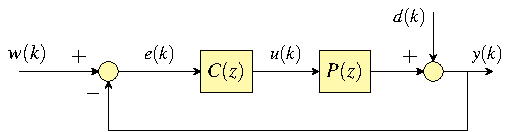
\includegraphics[width=0.50\columnwidth]{./Unit-04/img/ControlLoop-H1.pdf}
 \end{center}
 \begin{itemize}[<+-| alert@+>]
 \item The target transfer function is $G_{yw}(z)$, that we set equal to a desired $G_{yw}^{\circ}(z)$ writing
       \begin{displaymath} 
       \frac{P(z)C(z)}{1+P(z)C(z)} = G_{yw}^{\circ}(z).
       \end{displaymath}
 \item Solving for $C(z)$ we get
       \begin{displaymath} 
        C(z) = \frac{1}{P(z)} \, \frac{G_{yw}^{\circ}(z)}{1-G_{yw}^{\circ}(z)}.
       \end{displaymath}
 \item Note the cancellation (the $1/P$ factor in $C$).
 \end{itemize}
\end{frame}

\begin{frame}
\frametitleTC{Direct synthesis for disturbance rejection}
\framesubtitleTC{}
\myPause
 \begin{center}
  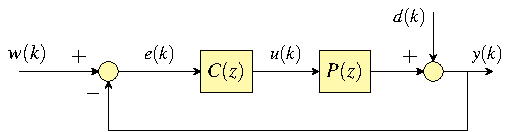
\includegraphics[width=0.50\columnwidth]{./Unit-04/img/ControlLoop-H1.pdf}
 \end{center}
 \begin{itemize}[<+-| alert@+>]
 \item The target transfer function is $G_{yd}(z)$, that we set equal to a desired $G_{yd}^{\circ}(z)$ writing
       \begin{displaymath} 
       \frac{1}{1+P(z)C(z)} = G_{yd}^{\circ}(z).
       \end{displaymath}
 \item Solving for $C(z)$ we get
       \begin{displaymath} 
        C(z) = \frac{1}{P(z)} \, \frac{1-G_{yd}^{\circ}(z)}{G_{yd}^{\circ}(z)}.
       \end{displaymath}
 \item Note the cancellation (the $1/P$ factor in $C$).
 \end{itemize}
\end{frame}

\begin{frame}\mccz
\frametitleTC{Direct synthesis}
\framesubtitleTC{Why ``PIDs on the horizon''?}
\myPause
 \begin{columns}
  \column[T]{0.35\textwidth}
   \only<2->{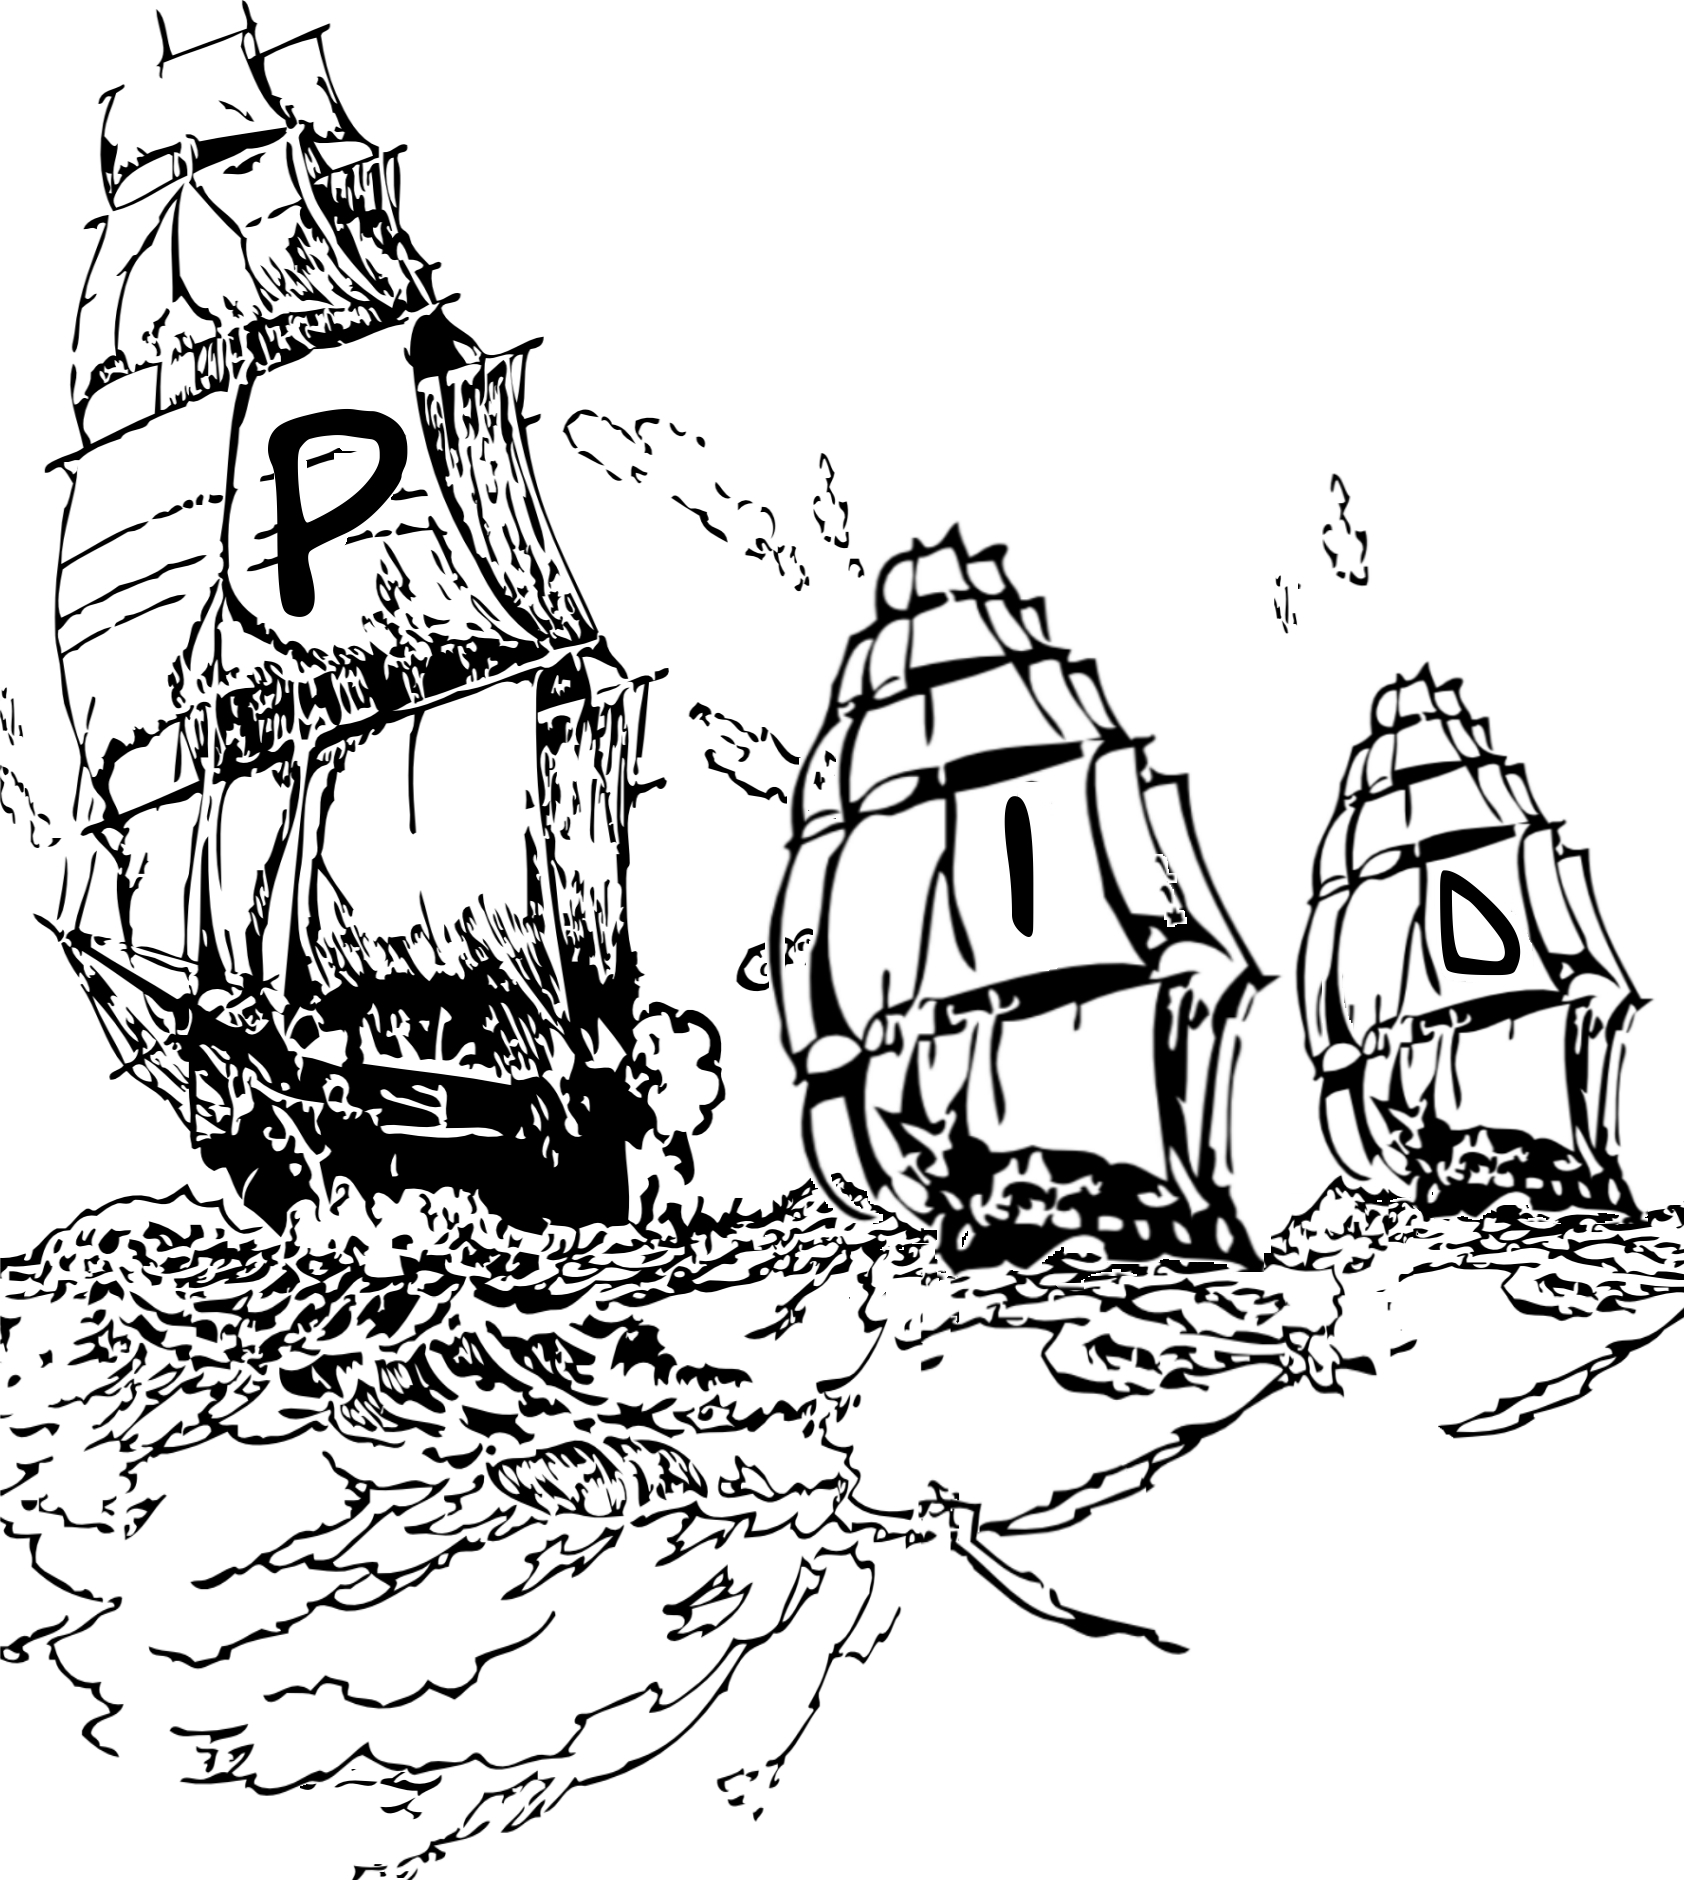
\includegraphics[height=6cm]{./Unit-04/img/PIDsOnTheHorizon_cc0.jpg}}
  \column[T]{0.65\textwidth}
   \begin{itemize}[<+-| alert@+>]
   \item Because applying direct synthesis to the versatile\\
         model we used to generate a variety of responses,\\
         with a sensible target transfer function, naturally\\
         leads to a controller with two zeroes and two\\
         poles, one of which in $z=1$.
   \item This is a PID controller.
   \item However we introduced a lot of material\\
         in this lecture.
   \item Better take a breath, recap, ad go\\
         through a practice session.
   \end{itemize}
 \end{columns}
\end{frame}




